% This file was created by tikzplotlib v0.8.2.
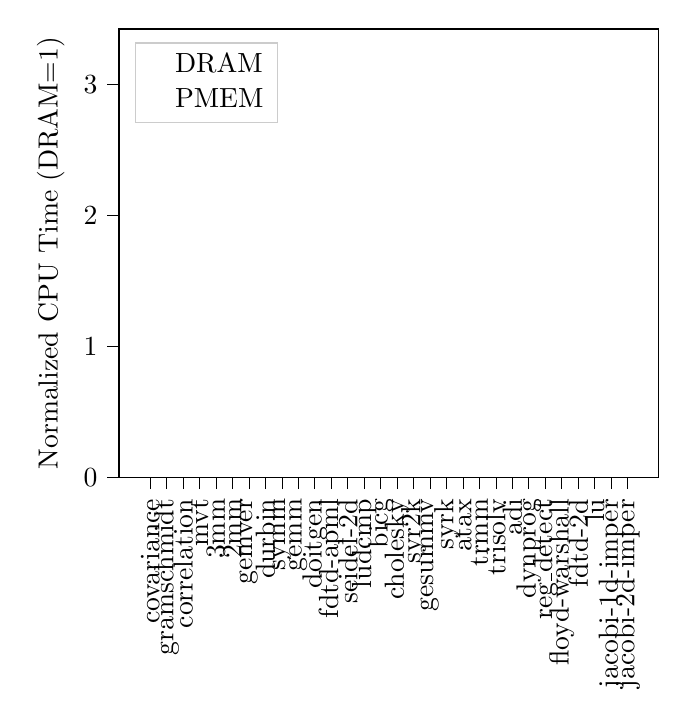
\begin{tikzpicture}

\begin{axis}[
legend cell align={left},
legend style={at={(0.03,0.97)}, anchor=north west, draw=white!80.0!black},
tick align=outside,
tick pos=left,
xmin=-1.69, xmax=31.09,
xtick style={color=black},
xtick={0.2,1.2,2.2,3.2,4.2,5.2,6.2,7.2,8.2,9.2,10.2,11.2,12.2,13.2,14.2,15.2,16.2,17.2,18.2,19.2,20.2,21.2,22.2,23.2,24.2,25.2,26.2,27.2,28.2,29.2},
xticklabel style = {rotate=90.0},
xticklabels={covariance,gramschmidt,correlation,mvt,3mm,2mm,gemver,durbin,symm,gemm,doitgen,fdtd-apml,seidel-2d,ludcmp,bicg,cholesky,syr2k,gesummv,syrk,atax,trmm,trisolv,adi,dynprog,reg\_detect,floyd-warshall,fdtd-2d,lu,jacobi-1d-imper,jacobi-2d-imper},
ylabel={Normalized CPU Time (DRAM=1)},
ymin=0, ymax=3.4227519480892,
ytick style={color=black}
]
\draw[fill=white,draw opacity=0,fill opacity=0.2,very thin] (axis cs:-0.2,0) rectangle (axis cs:0.2,1);
\addlegendimage{ybar,ybar legend,fill=white,draw opacity=0,fill opacity=0.2,very thin};
\addlegendentry{DRAM}

\draw[fill=white,draw opacity=0,fill opacity=0.2,very thin] (axis cs:0.8,0) rectangle (axis cs:1.2,1);
\draw[fill=white,draw opacity=0,fill opacity=0.2,very thin] (axis cs:1.8,0) rectangle (axis cs:2.2,1);
\draw[fill=white,draw opacity=0,fill opacity=0.2,very thin] (axis cs:2.8,0) rectangle (axis cs:3.2,1);
\draw[fill=white,draw opacity=0,fill opacity=0.2,very thin] (axis cs:3.8,0) rectangle (axis cs:4.2,1);
\draw[fill=white,draw opacity=0,fill opacity=0.2,very thin] (axis cs:4.8,0) rectangle (axis cs:5.2,1);
\draw[fill=white,draw opacity=0,fill opacity=0.2,very thin] (axis cs:5.8,0) rectangle (axis cs:6.2,1);
\draw[fill=white,draw opacity=0,fill opacity=0.2,very thin] (axis cs:6.8,0) rectangle (axis cs:7.2,1);
\draw[fill=white,draw opacity=0,fill opacity=0.2,very thin] (axis cs:7.8,0) rectangle (axis cs:8.2,1);
\draw[fill=white,draw opacity=0,fill opacity=0.2,very thin] (axis cs:8.8,0) rectangle (axis cs:9.2,1);
\draw[fill=white,draw opacity=0,fill opacity=0.2,very thin] (axis cs:9.8,0) rectangle (axis cs:10.2,1);
\draw[fill=white,draw opacity=0,fill opacity=0.2,very thin] (axis cs:10.8,0) rectangle (axis cs:11.2,1);
\draw[fill=white,draw opacity=0,fill opacity=0.2,very thin] (axis cs:11.8,0) rectangle (axis cs:12.2,1);
\draw[fill=white,draw opacity=0,fill opacity=0.2,very thin] (axis cs:12.8,0) rectangle (axis cs:13.2,1);
\draw[fill=white,draw opacity=0,fill opacity=0.2,very thin] (axis cs:13.8,0) rectangle (axis cs:14.2,1);
\draw[fill=white,draw opacity=0,fill opacity=0.2,very thin] (axis cs:14.8,0) rectangle (axis cs:15.2,1);
\draw[fill=white,draw opacity=0,fill opacity=0.2,very thin] (axis cs:15.8,0) rectangle (axis cs:16.2,1);
\draw[fill=white,draw opacity=0,fill opacity=0.2,very thin] (axis cs:16.8,0) rectangle (axis cs:17.2,1);
\draw[fill=white,draw opacity=0,fill opacity=0.2,very thin] (axis cs:17.8,0) rectangle (axis cs:18.2,1);
\draw[fill=white,draw opacity=0,fill opacity=0.2,very thin] (axis cs:18.8,0) rectangle (axis cs:19.2,1);
\draw[fill=white,draw opacity=0,fill opacity=0.2,very thin] (axis cs:19.8,0) rectangle (axis cs:20.2,1);
\draw[fill=white,draw opacity=0,fill opacity=0.2,very thin] (axis cs:20.8,0) rectangle (axis cs:21.2,1);
\draw[fill=white,draw opacity=0,fill opacity=0.2,very thin] (axis cs:21.8,0) rectangle (axis cs:22.2,1);
\draw[fill=white,draw opacity=0,fill opacity=0.2,very thin] (axis cs:22.8,0) rectangle (axis cs:23.2,1);
\draw[fill=white,draw opacity=0,fill opacity=0.2,very thin] (axis cs:23.8,0) rectangle (axis cs:24.2,1);
\draw[fill=white,draw opacity=0,fill opacity=0.2,very thin] (axis cs:24.8,0) rectangle (axis cs:25.2,1);
\draw[fill=white,draw opacity=0,fill opacity=0.2,very thin] (axis cs:25.8,0) rectangle (axis cs:26.2,1);
\draw[fill=white,draw opacity=0,fill opacity=0.2,very thin] (axis cs:26.8,0) rectangle (axis cs:27.2,1);
\draw[fill=white,draw opacity=0,fill opacity=0.2,very thin] (axis cs:27.8,0) rectangle (axis cs:28.2,1);
\draw[fill=white,draw opacity=0,fill opacity=0.2,very thin] (axis cs:28.8,0) rectangle (axis cs:29.2,1);
\draw[fill=white,draw opacity=0,fill opacity=0.2,very thin] (axis cs:0.2,0) rectangle (axis cs:0.6,0.20790754294425);
\addlegendimage{ybar,ybar legend,fill=white,draw opacity=0,fill opacity=0.2,very thin};
\addlegendentry{PMEM}

\draw[fill=white,draw opacity=0,fill opacity=0.2,very thin] (axis cs:1.2,0) rectangle (axis cs:1.6,0.248193661771417);
\draw[fill=white,draw opacity=0,fill opacity=0.2,very thin] (axis cs:2.2,0) rectangle (axis cs:2.6,0.379546198041494);
\draw[fill=white,draw opacity=0,fill opacity=0.2,very thin] (axis cs:3.2,0) rectangle (axis cs:3.6,0.616774349886283);
\draw[fill=white,draw opacity=0,fill opacity=0.2,very thin] (axis cs:4.2,0) rectangle (axis cs:4.6,0.686413716946976);
\draw[fill=white,draw opacity=0,fill opacity=0.2,very thin] (axis cs:5.2,0) rectangle (axis cs:5.6,0.72418682235196);
\draw[fill=white,draw opacity=0,fill opacity=0.2,very thin] (axis cs:6.2,0) rectangle (axis cs:6.6,0.740789764860638);
\draw[fill=white,draw opacity=0,fill opacity=0.2,very thin] (axis cs:7.2,0) rectangle (axis cs:7.6,0.75449090357582);
\draw[fill=white,draw opacity=0,fill opacity=0.2,very thin] (axis cs:8.2,0) rectangle (axis cs:8.6,0.762677303103743);
\draw[fill=white,draw opacity=0,fill opacity=0.2,very thin] (axis cs:9.2,0) rectangle (axis cs:9.6,0.940082255924022);
\draw[fill=white,draw opacity=0,fill opacity=0.2,very thin] (axis cs:10.2,0) rectangle (axis cs:10.6,0.959591331531782);
\draw[fill=white,draw opacity=0,fill opacity=0.2,very thin] (axis cs:11.2,0) rectangle (axis cs:11.6,0.997193635258573);
\draw[fill=white,draw opacity=0,fill opacity=0.2,very thin] (axis cs:12.2,0) rectangle (axis cs:12.6,1.00037667891458);
\draw[fill=white,draw opacity=0,fill opacity=0.2,very thin] (axis cs:13.2,0) rectangle (axis cs:13.6,1.04337148158142);
\draw[fill=white,draw opacity=0,fill opacity=0.2,very thin] (axis cs:14.2,0) rectangle (axis cs:14.6,1.32198186951709);
\draw[fill=white,draw opacity=0,fill opacity=0.2,very thin] (axis cs:15.2,0) rectangle (axis cs:15.6,1.43864236849485);
\draw[fill=white,draw opacity=0,fill opacity=0.2,very thin] (axis cs:16.2,0) rectangle (axis cs:16.6,1.44935495159561);
\draw[fill=white,draw opacity=0,fill opacity=0.2,very thin] (axis cs:17.2,0) rectangle (axis cs:17.6,1.57716076845298);
\draw[fill=white,draw opacity=0,fill opacity=0.2,very thin] (axis cs:18.2,0) rectangle (axis cs:18.6,1.66443299572832);
\draw[fill=white,draw opacity=0,fill opacity=0.2,very thin] (axis cs:19.2,0) rectangle (axis cs:19.6,1.79418024435724);
\draw[fill=white,draw opacity=0,fill opacity=0.2,very thin] (axis cs:20.2,0) rectangle (axis cs:20.6,1.83707479857955);
\draw[fill=white,draw opacity=0,fill opacity=0.2,very thin] (axis cs:21.2,0) rectangle (axis cs:21.6,2.00460329992372);
\draw[fill=white,draw opacity=0,fill opacity=0.2,very thin] (axis cs:22.2,0) rectangle (axis cs:22.6,2.79289079997318);
\draw[fill=white,draw opacity=0,fill opacity=0.2,very thin] (axis cs:23.2,0) rectangle (axis cs:23.6,2.82558652749306);
\draw[fill=white,draw opacity=0,fill opacity=0.2,very thin] (axis cs:24.2,0) rectangle (axis cs:24.6,3.07208804892073);
\draw[fill=white,draw opacity=0,fill opacity=0.2,very thin] (axis cs:25.2,0) rectangle (axis cs:25.6,3.07553662128085);
\draw[fill=white,draw opacity=0,fill opacity=0.2,very thin] (axis cs:26.2,0) rectangle (axis cs:26.6,3.14809152284577);
\draw[fill=white,draw opacity=0,fill opacity=0.2,very thin] (axis cs:27.2,0) rectangle (axis cs:27.6,3.19732984457504);
\draw[fill=white,draw opacity=0,fill opacity=0.2,very thin] (axis cs:28.2,0) rectangle (axis cs:28.6,3.2152462046701);
\draw[fill=white,draw opacity=0,fill opacity=0.2,very thin] (axis cs:29.2,0) rectangle (axis cs:29.6,3.25976376008495);
\end{axis}

\end{tikzpicture}